\documentclass[11pt]{article}
\usepackage[a4paper, margin=0.8in]{geometry}
\usepackage{tikz}
\usetikzlibrary{shapes.geometric, arrows.meta, positioning, shadows, backgrounds, fit, calc}
\usepackage{xcolor}
\usepackage{helvet}
\usepackage{amsmath}
\renewcommand{\familydefault}{\sfdefault}

\definecolor{bglight}{RGB}{248, 250, 252}
\definecolor{darkblue}{RGB}{15, 23, 42}
\definecolor{brandblue}{RGB}{37, 99, 235}
\definecolor{brandgreen}{RGB}{5, 150, 105}
\definecolor{boxfill}{RGB}{255, 255, 255}

\begin{document}
\pagecolor{bglight}

\noindent
\begin{tikzpicture}[remember picture, overlay]
    \fill[darkblue] (current page.north west) rectangle ([yshift=-3.5cm]current page.north east);
    \node[text=white, anchor=north west, font=\Huge\bfseries] at ([xshift=1.5cm, yshift=-1.2cm]current page.north west) {PySpectrometer2};
    \node[text=white, anchor=north west, font=\Large] at ([xshift=1.5cm, yshift=-2.2cm]current page.north west) {Conditional Multi-Axis Processing Architecture};
\end{tikzpicture}

\vspace{2.5cm}

\begin{center}
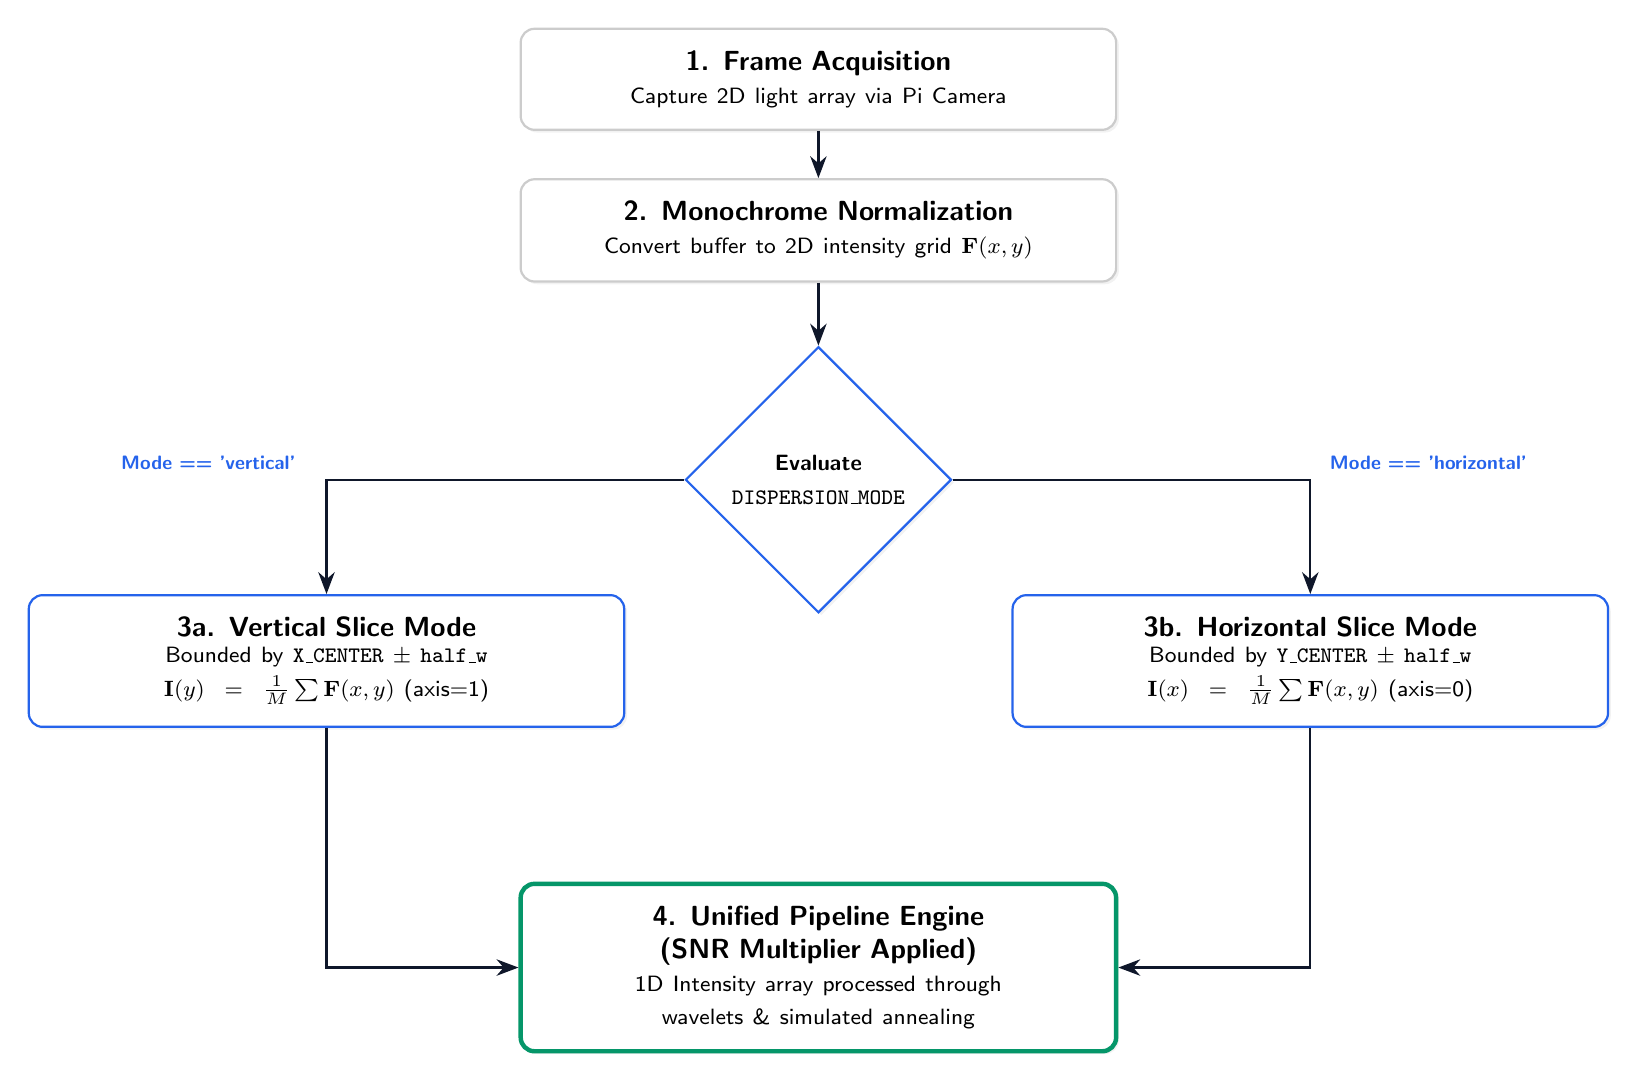
\begin{tikzpicture}[
    node distance=0.6cm and 0.8cm,
    base/.style={rectangle, rounded corners=5pt, draw=black!20, thick, fill=boxfill, text width=7.0cm, align=center, inner sep=8pt, drop shadow={opacity=0.1, shadow xshift=1pt, shadow yshift=-1pt}},
    decision/.style={diamond, draw=brandblue, thick, fill=boxfill, text width=2.2cm, align=center, inner sep=4pt, drop shadow={opacity=0.1, shadow xshift=1pt, shadow yshift=-1pt}},
    arrow/.style={-{Stealth[scale=1.2]}, thick, color=darkblue},
    labelnode/.style={font=\scriptsize\bfseries, color=brandblue}
]

% Main Spine
\node (hardware) [base] {\textbf{1. Frame Acquisition} \\ \footnotesize Capture 2D light array via Pi Camera};
\node (pre) [base, below=of hardware] {\textbf{2. Monochrome Normalization} \\ \footnotesize Convert buffer to 2D intensity grid $\mathbf{F}(x,y)$};

% Decision Diamond
\node (decide) [decision, below=of pre, yshift=-0.2cm] {\footnotesize \textbf{Evaluate}\\ \texttt{DISPERSION\_MODE}};

% Branches
\node (vert) [base, below left=of decide, xshift=-0.8cm, draw=brandblue] {
    \textbf{3a. Vertical Slice Mode}\\
    \footnotesize Bounded by \texttt{X\_CENTER} $\pm$ \texttt{half\_w}\\
    \footnotesize $\mathbf{I}(y) = \frac{1}{M}\sum \mathbf{F}(x,y)$ (axis=1)
};

\node (horiz) [base, below right=of decide, xshift=0.8cm, draw=brandblue] {
    \textbf{3b. Horizontal Slice Mode}\\
    \footnotesize Bounded by \texttt{Y\_CENTER} $\pm$ \texttt{half\_w}\\
    \footnotesize $\mathbf{I}(x) = \frac{1}{M}\sum \mathbf{F}(x,y)$ (axis=0)
};

% Re-convergence point
\node (math) [base, below=of decide, yshift=-2.8cm, draw=brandgreen, ultra thick] {
    \textbf{4. Unified Pipeline Engine (SNR Multiplier Applied)}\\
    \footnotesize 1D Intensity array processed through wavelets \& simulated annealing
};

% Connections
\draw [arrow] (hardware) -- (pre);
\draw [arrow] (pre) -- (decide);
\draw [arrow] (decide) -| node[above, xshift=-1.5cm, labelnode] {Mode == 'vertical'} (vert);
\draw [arrow] (decide) -| node[above, xshift=1.5cm, labelnode] {Mode == 'horizontal'} (horiz);
\draw [arrow] (vert) |- (math);
\draw [arrow] (horiz) |- (math);

\end{tikzpicture}
\end{center}

\end{document}
